\question (北京邮电大学,2002年)流水CPU是由一系列叫做``段''的处理线路所组成的。和具有m个并行部件的CPU相比,一个m段流水线CPU
\par\twoch{\textcolor{red}{具有同等水平的吞吐能力}}{不具备同等水平的吞吐能力}{吞吐能力大于前者的吞吐能力}{吞吐能力小于前者的吞吐能力}
\begin{solution}一个m段流水线CPU和具有m个并行部件的CPU相比具有同等水平的吞吐能力。
\end{solution}
\question 某CPU主频为1.03GHz,采用4级指令流水线,每个流水段的执行需要1个时钟周期。假定CPU执行了100条指令,在其执行过程中,没有发生任何流水线阻塞,此时流水线的吞吐率为(
)
\par\fourch{$0.25×10^9$条指令/秒}{$0.97×10^9$条指令/秒}{\textcolor{red}{$1.0×10^9$条指令/秒}}{$1.03×10^9$条指令/秒}
\begin{solution}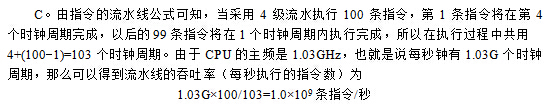
\includegraphics[width=5.73958in,height=1.09375in]{computerassets/7e707ae279824ceb7945f57d5c919616.jpeg}
\end{solution}
